\documentclass[12pt, a4paper, twoside]{article}

\usepackage{graphicx}
\usepackage[a4paper, left=2cm, right=2cm, top=2.5cm, bottom=3cm]{geometry}
\usepackage{float}
\usepackage[ngerman]{babel}

\begin{document}
    \thispagestyle{empty}
     \vspace*{4cm}
    \begin{center}
        \includegraphics[width=200pt]{Bilder/Helmut Schmidt Universität-a89973ff.png}\\
        \vspace{2cm}
        \huge\textbf{MATLAB - Grundlagen für Ingenieurwissenschaften}
    \end{center}
    \newpage

    \pagenumbering{arabic}
    \renewcommand{\contentsname}{Inhaltsverzeichnis}
    \tableofcontents
    \newpage
    \section{Einführung}
        \subsection{Was ist MATLAB}
        MATLAB ist die Abkürzung für MATrix LABoratory. Zudem ist es ein interaktives, integriertes System zur Berechnung, Visualisierung oder Programmierung mathematischer Problemstellungen. Es bietet eine einfache Skriptsprache welche auf die Verarbeitung von Matrizen ausgelegt ist.
        \subsection{Anwendungsgebiete in den Ingenieurwissenschaften}
        MATLAB bietet in vielen Ingenieurwissenschaftlichen Betätigungsfeldern weitreichende \\Vorteile.
        \begin{itemize}
            \item Signalverarbeitung
            \item Regelungstechnik
            \item FEM-Simulation
            \item Schaltungsanalyse
            \item Bildverarbeitung
            \item Datenanalyse
        \end{itemize}
        \subsection{Die Benutzeroberfläche}
            \subsubsection*{Command Window}
                \begin{figure}[H]
                    \centering
                    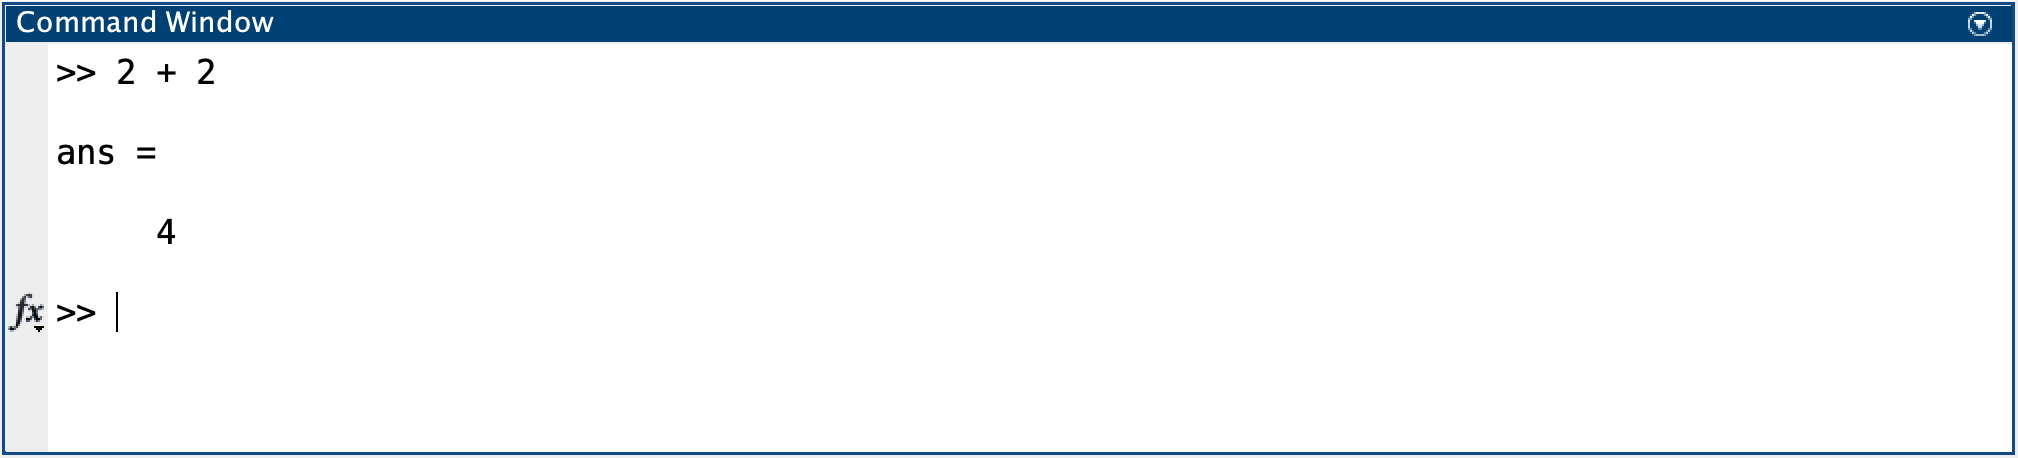
\includegraphics[width=0.7\textwidth]{Bilder/CommandWindow.png}
                    \caption{Command Window in MATLAB}
                \end{figure}
                Im Command Window können Befehle direkt eingegeben werden. Da Ergebnisse von Berechnungen unverzüglich angezeigt werden, können hier einzelne Befehle idealerweise getestet werden.
            \subsubsection*{Editor}
                \begin{figure}[H]
                    \centering
                    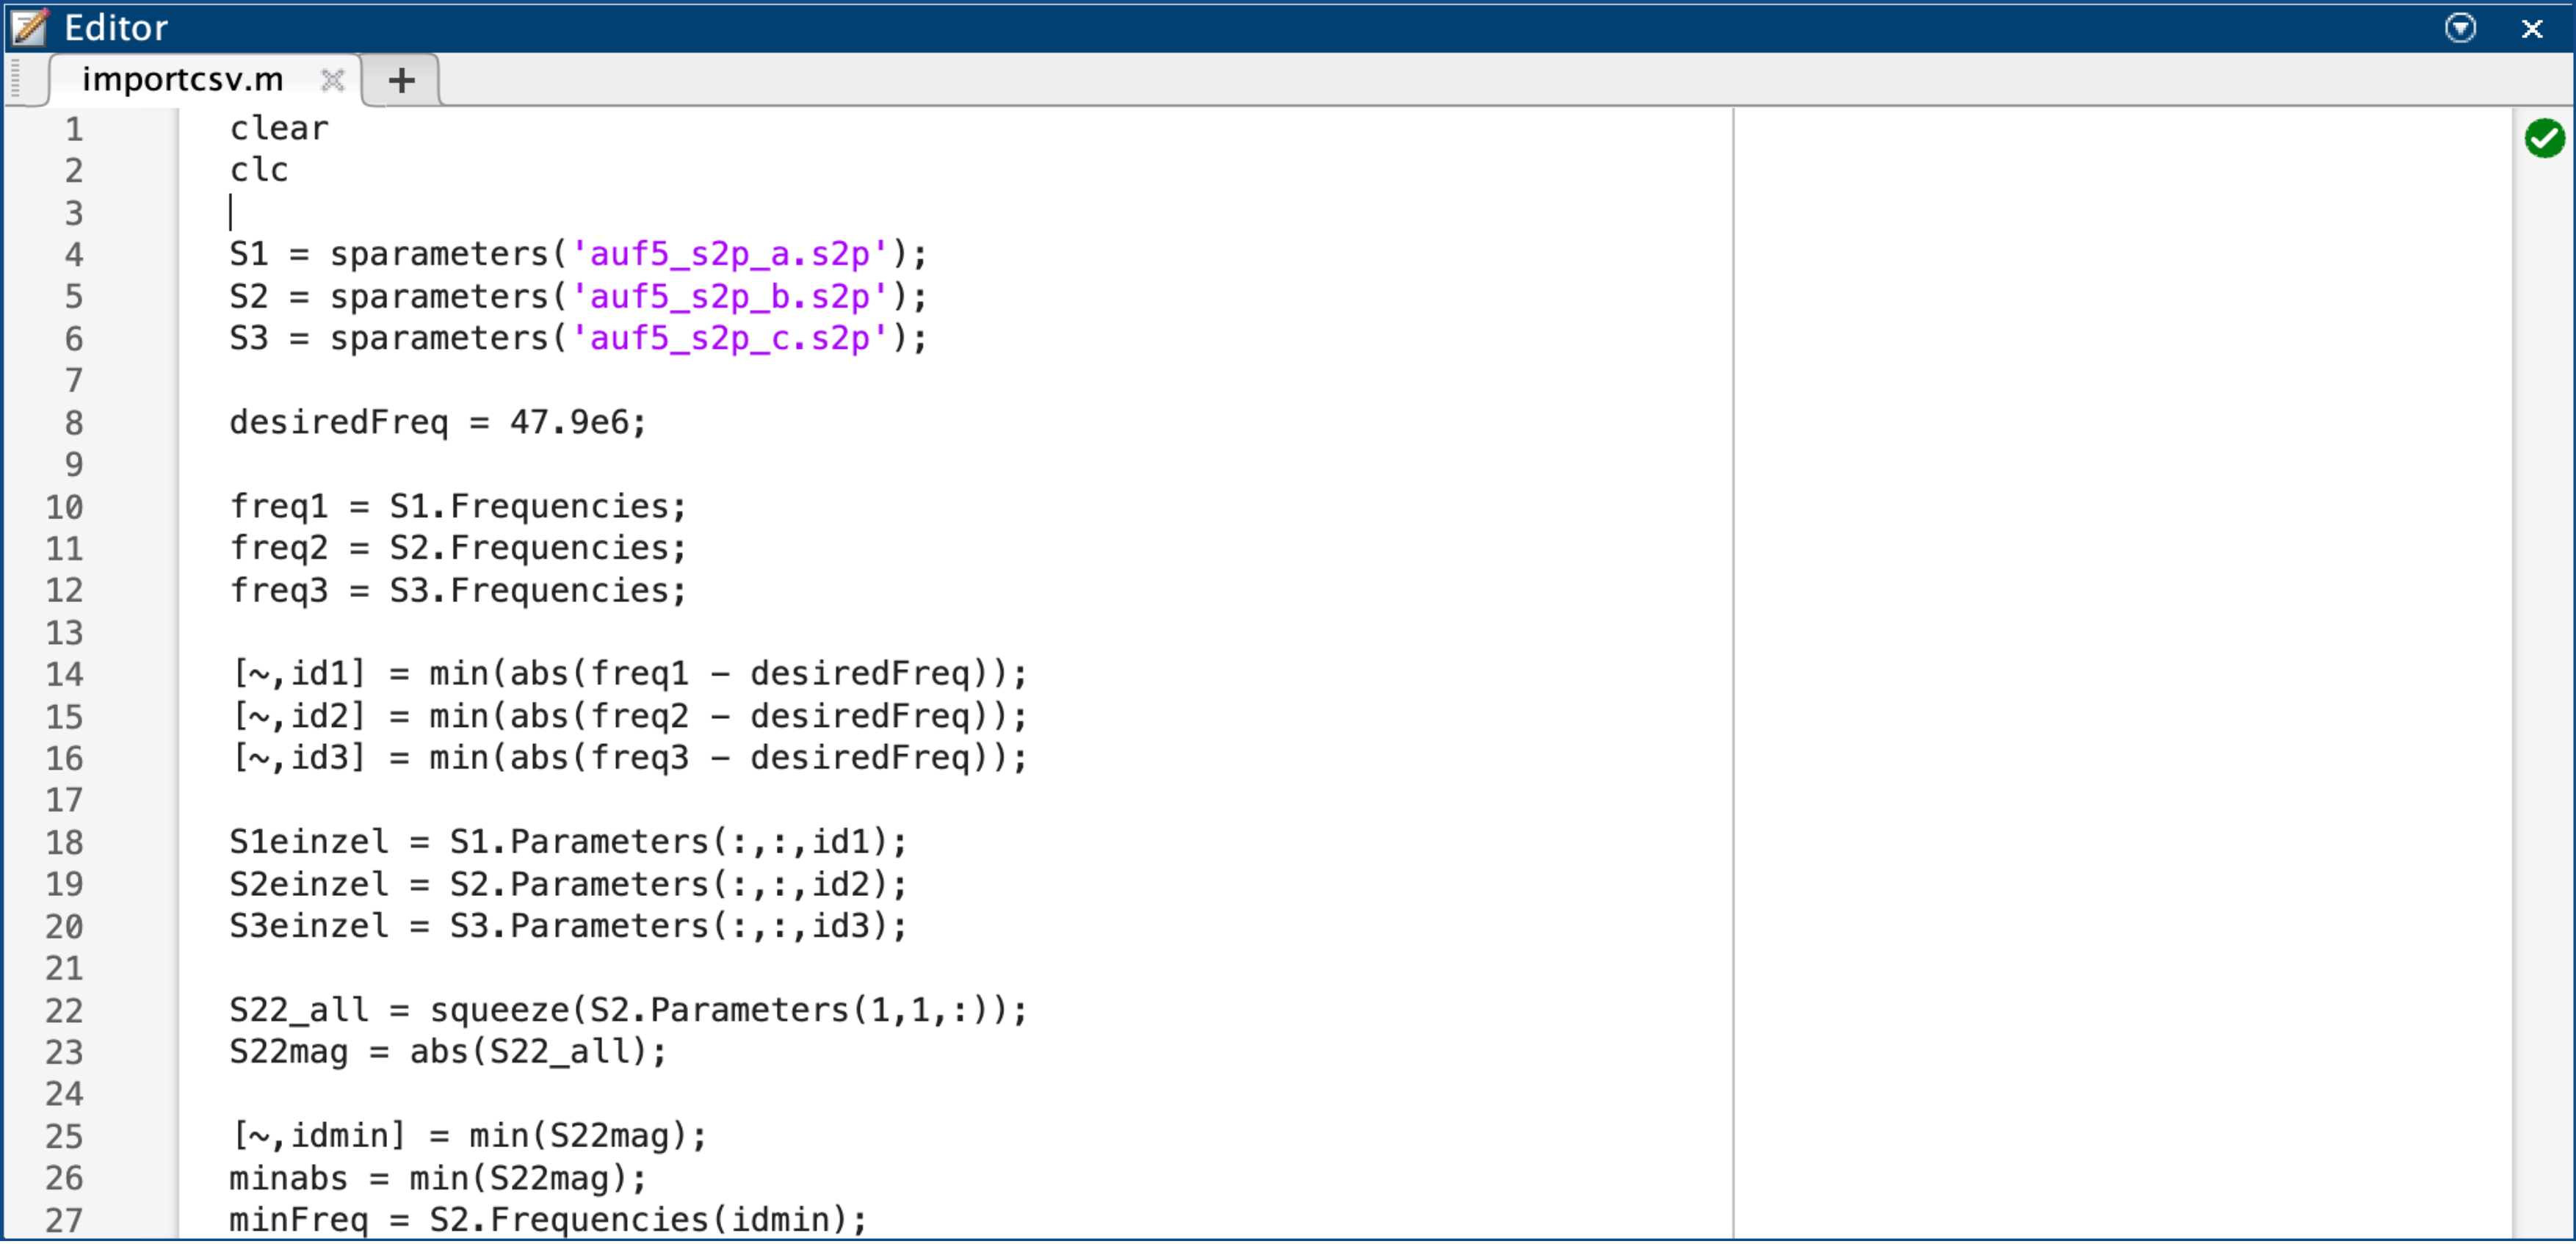
\includegraphics[width=0.7\textwidth]{Bilder/Editor.png}
                    \caption{Editor in MATLAB}
                \end{figure}
                Im Editor können komplette Skripte und Funktionen geschrieben, gespeichert und ausgeführt werden. Er unterstützt das Debugging mittels Breakpoints und Schritt-für-Schritt Ausführung.
            \subsubsection*{Workspace}
                \begin{figure}[H]
                    \centering
                    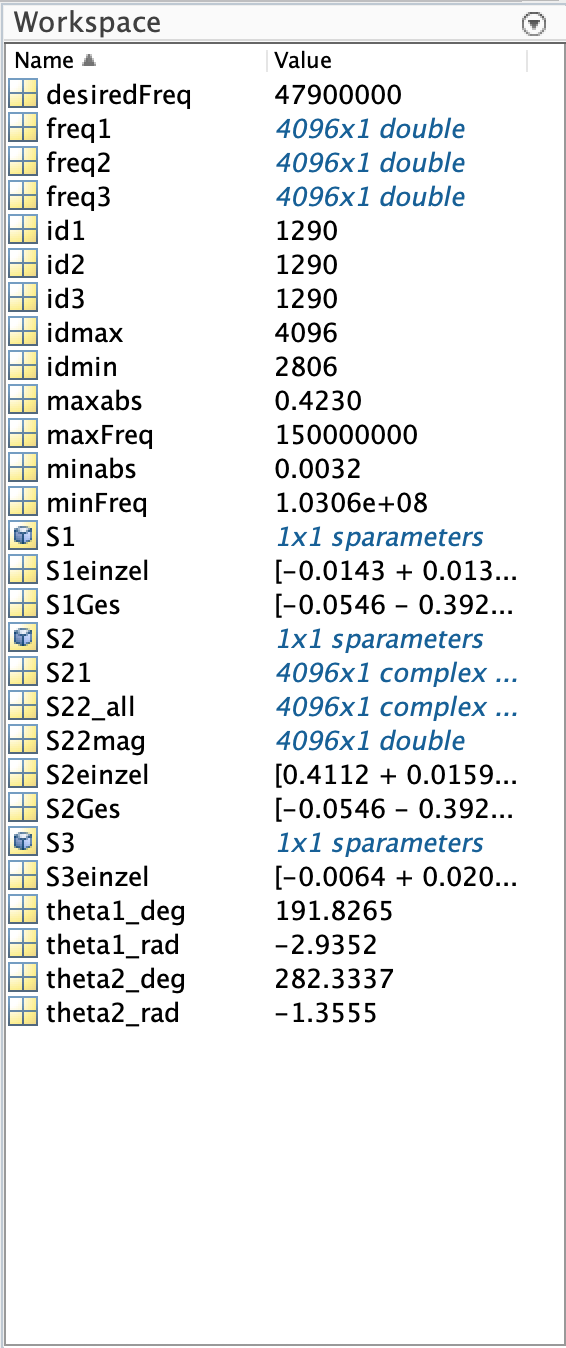
\includegraphics[width=0.2\textwidth]{Bilder/Workspace.png}
                    \caption{Workspace in MATLAB}
                \end{figure}
                Im Workspace werden alle aktuellen Variablen inklusive ihres Inhalts angezeigt. Weiterhin ist es möglich diese Variablen hier manuell anzupassen oder zu löschen.
            \subsubsection*{Current Folder}
                \begin{figure}[H]
                    \centering
                    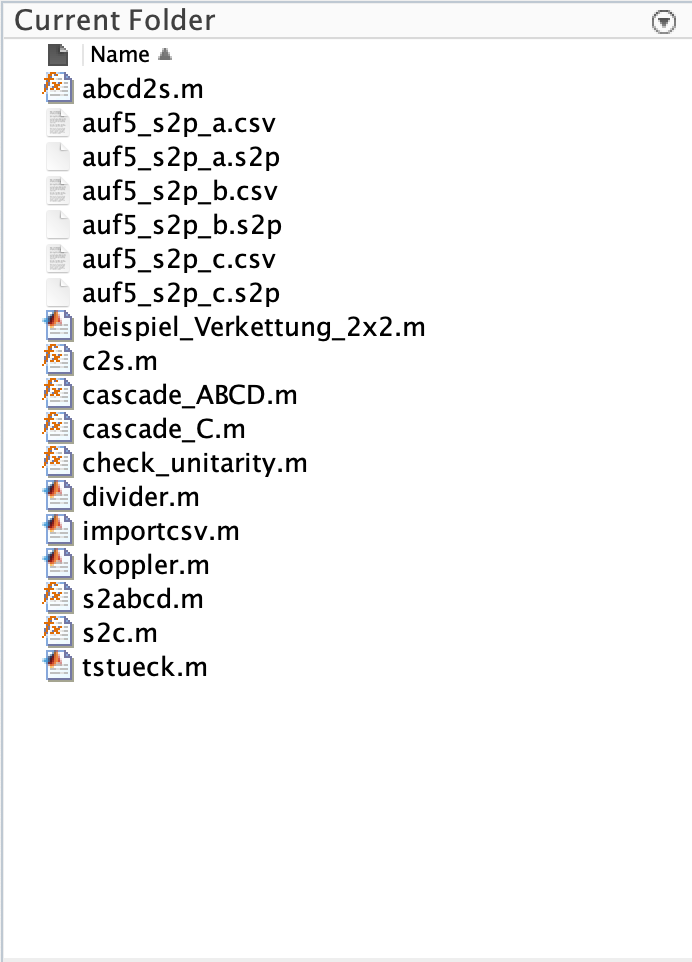
\includegraphics[width=0.3\textwidth]{Bilder/CurrentFolder.png}      
                    \caption{Current Folder in MATLAB}              
                \end{figure}
                Im Current Folder findet man alle Dateien des Projektordners. Diese können durch Doppelklick oder das Ziehen in den Editor geöffnet und bearbeitet werden.
            \newpage
            
    \section{Grundlegende Operationen}
        \subsection{Variablendeklaration}
        \subsection{Mathematische Grundoperationen}
        \subsection{Kommentare}
        \subsection{Komplexe Zahlen}
    \section{Vektoren und Matrizen}
        \subsection{Erstellen von Vektoren und Matrizen}
        \subsection{Zugriff auf Elemente und Indizierung}
        \subsection{Matrixoperationen}
        \subsection{nützliche MATLAB Funktionen}
    \section{Programmiergrundlagen}
        \subsection{Skripte}
        \subsection{Funktionen}
        \subsection{Schleifen}
    \section{Arbeiten mit Dateien und Daten}
        \subsection{Speichern und Laden von Daten}
        \subsection{Importieren von Messdaten}
        \subsection{Analyse und Verarbeitung von Daten}
    \section{Visualisierung von Daten}
        \subsection{Einfache Diagramme}
        \subsection{Mehrere Kurven in einem Diagramm}
        \subsection{Mehrere Diagramme in einer Übersicht}
        \subsection{Grafische Anpassungen}
    \section{Anhang}
        \subsection{Dokumentation in MATLAB}
        \subsection{Übersicht wichtiger MATLAB Befehle}
\end{document}
